% Options for packages loaded elsewhere
\PassOptionsToPackage{unicode}{hyperref}
\PassOptionsToPackage{hyphens}{url}
\PassOptionsToPackage{dvipsnames,svgnames,x11names}{xcolor}
%
\documentclass[
  letterpaper,
  DIV=11,
  numbers=noendperiod]{scrartcl}

\usepackage{amsmath,amssymb}
\usepackage{iftex}
\ifPDFTeX
  \usepackage[T1]{fontenc}
  \usepackage[utf8]{inputenc}
  \usepackage{textcomp} % provide euro and other symbols
\else % if luatex or xetex
  \usepackage{unicode-math}
  \defaultfontfeatures{Scale=MatchLowercase}
  \defaultfontfeatures[\rmfamily]{Ligatures=TeX,Scale=1}
\fi
\usepackage{lmodern}
\ifPDFTeX\else  
    % xetex/luatex font selection
\fi
% Use upquote if available, for straight quotes in verbatim environments
\IfFileExists{upquote.sty}{\usepackage{upquote}}{}
\IfFileExists{microtype.sty}{% use microtype if available
  \usepackage[]{microtype}
  \UseMicrotypeSet[protrusion]{basicmath} % disable protrusion for tt fonts
}{}
\makeatletter
\@ifundefined{KOMAClassName}{% if non-KOMA class
  \IfFileExists{parskip.sty}{%
    \usepackage{parskip}
  }{% else
    \setlength{\parindent}{0pt}
    \setlength{\parskip}{6pt plus 2pt minus 1pt}}
}{% if KOMA class
  \KOMAoptions{parskip=half}}
\makeatother
\usepackage{xcolor}
\usepackage[margin=1in]{geometry}
\setlength{\emergencystretch}{3em} % prevent overfull lines
\setcounter{secnumdepth}{-\maxdimen} % remove section numbering
% Make \paragraph and \subparagraph free-standing
\makeatletter
\ifx\paragraph\undefined\else
  \let\oldparagraph\paragraph
  \renewcommand{\paragraph}{
    \@ifstar
      \xxxParagraphStar
      \xxxParagraphNoStar
  }
  \newcommand{\xxxParagraphStar}[1]{\oldparagraph*{#1}\mbox{}}
  \newcommand{\xxxParagraphNoStar}[1]{\oldparagraph{#1}\mbox{}}
\fi
\ifx\subparagraph\undefined\else
  \let\oldsubparagraph\subparagraph
  \renewcommand{\subparagraph}{
    \@ifstar
      \xxxSubParagraphStar
      \xxxSubParagraphNoStar
  }
  \newcommand{\xxxSubParagraphStar}[1]{\oldsubparagraph*{#1}\mbox{}}
  \newcommand{\xxxSubParagraphNoStar}[1]{\oldsubparagraph{#1}\mbox{}}
\fi
\makeatother

\usepackage{color}
\usepackage{fancyvrb}
\newcommand{\VerbBar}{|}
\newcommand{\VERB}{\Verb[commandchars=\\\{\}]}
\DefineVerbatimEnvironment{Highlighting}{Verbatim}{commandchars=\\\{\}}
% Add ',fontsize=\small' for more characters per line
\usepackage{framed}
\definecolor{shadecolor}{RGB}{241,243,245}
\newenvironment{Shaded}{\begin{snugshade}}{\end{snugshade}}
\newcommand{\AlertTok}[1]{\textcolor[rgb]{0.68,0.00,0.00}{#1}}
\newcommand{\AnnotationTok}[1]{\textcolor[rgb]{0.37,0.37,0.37}{#1}}
\newcommand{\AttributeTok}[1]{\textcolor[rgb]{0.40,0.45,0.13}{#1}}
\newcommand{\BaseNTok}[1]{\textcolor[rgb]{0.68,0.00,0.00}{#1}}
\newcommand{\BuiltInTok}[1]{\textcolor[rgb]{0.00,0.23,0.31}{#1}}
\newcommand{\CharTok}[1]{\textcolor[rgb]{0.13,0.47,0.30}{#1}}
\newcommand{\CommentTok}[1]{\textcolor[rgb]{0.37,0.37,0.37}{#1}}
\newcommand{\CommentVarTok}[1]{\textcolor[rgb]{0.37,0.37,0.37}{\textit{#1}}}
\newcommand{\ConstantTok}[1]{\textcolor[rgb]{0.56,0.35,0.01}{#1}}
\newcommand{\ControlFlowTok}[1]{\textcolor[rgb]{0.00,0.23,0.31}{\textbf{#1}}}
\newcommand{\DataTypeTok}[1]{\textcolor[rgb]{0.68,0.00,0.00}{#1}}
\newcommand{\DecValTok}[1]{\textcolor[rgb]{0.68,0.00,0.00}{#1}}
\newcommand{\DocumentationTok}[1]{\textcolor[rgb]{0.37,0.37,0.37}{\textit{#1}}}
\newcommand{\ErrorTok}[1]{\textcolor[rgb]{0.68,0.00,0.00}{#1}}
\newcommand{\ExtensionTok}[1]{\textcolor[rgb]{0.00,0.23,0.31}{#1}}
\newcommand{\FloatTok}[1]{\textcolor[rgb]{0.68,0.00,0.00}{#1}}
\newcommand{\FunctionTok}[1]{\textcolor[rgb]{0.28,0.35,0.67}{#1}}
\newcommand{\ImportTok}[1]{\textcolor[rgb]{0.00,0.46,0.62}{#1}}
\newcommand{\InformationTok}[1]{\textcolor[rgb]{0.37,0.37,0.37}{#1}}
\newcommand{\KeywordTok}[1]{\textcolor[rgb]{0.00,0.23,0.31}{\textbf{#1}}}
\newcommand{\NormalTok}[1]{\textcolor[rgb]{0.00,0.23,0.31}{#1}}
\newcommand{\OperatorTok}[1]{\textcolor[rgb]{0.37,0.37,0.37}{#1}}
\newcommand{\OtherTok}[1]{\textcolor[rgb]{0.00,0.23,0.31}{#1}}
\newcommand{\PreprocessorTok}[1]{\textcolor[rgb]{0.68,0.00,0.00}{#1}}
\newcommand{\RegionMarkerTok}[1]{\textcolor[rgb]{0.00,0.23,0.31}{#1}}
\newcommand{\SpecialCharTok}[1]{\textcolor[rgb]{0.37,0.37,0.37}{#1}}
\newcommand{\SpecialStringTok}[1]{\textcolor[rgb]{0.13,0.47,0.30}{#1}}
\newcommand{\StringTok}[1]{\textcolor[rgb]{0.13,0.47,0.30}{#1}}
\newcommand{\VariableTok}[1]{\textcolor[rgb]{0.07,0.07,0.07}{#1}}
\newcommand{\VerbatimStringTok}[1]{\textcolor[rgb]{0.13,0.47,0.30}{#1}}
\newcommand{\WarningTok}[1]{\textcolor[rgb]{0.37,0.37,0.37}{\textit{#1}}}

\providecommand{\tightlist}{%
  \setlength{\itemsep}{0pt}\setlength{\parskip}{0pt}}\usepackage{longtable,booktabs,array}
\usepackage{calc} % for calculating minipage widths
% Correct order of tables after \paragraph or \subparagraph
\usepackage{etoolbox}
\makeatletter
\patchcmd\longtable{\par}{\if@noskipsec\mbox{}\fi\par}{}{}
\makeatother
% Allow footnotes in longtable head/foot
\IfFileExists{footnotehyper.sty}{\usepackage{footnotehyper}}{\usepackage{footnote}}
\makesavenoteenv{longtable}
\usepackage{graphicx}
\makeatletter
\newsavebox\pandoc@box
\newcommand*\pandocbounded[1]{% scales image to fit in text height/width
  \sbox\pandoc@box{#1}%
  \Gscale@div\@tempa{\textheight}{\dimexpr\ht\pandoc@box+\dp\pandoc@box\relax}%
  \Gscale@div\@tempb{\linewidth}{\wd\pandoc@box}%
  \ifdim\@tempb\p@<\@tempa\p@\let\@tempa\@tempb\fi% select the smaller of both
  \ifdim\@tempa\p@<\p@\scalebox{\@tempa}{\usebox\pandoc@box}%
  \else\usebox{\pandoc@box}%
  \fi%
}
% Set default figure placement to htbp
\def\fps@figure{htbp}
\makeatother

\usepackage{booktabs}
\usepackage{longtable}
\usepackage{array}
\usepackage{multirow}
\usepackage{wrapfig}
\usepackage{float}
\usepackage{colortbl}
\usepackage{pdflscape}
\usepackage{tabu}
\usepackage{threeparttable}
\usepackage{threeparttablex}
\usepackage[normalem]{ulem}
\usepackage{makecell}
\usepackage{xcolor}
\KOMAoption{captions}{tableheading,figureheading}
\makeatletter
\@ifpackageloaded{caption}{}{\usepackage{caption}}
\AtBeginDocument{%
\ifdefined\contentsname
  \renewcommand*\contentsname{Table of contents}
\else
  \newcommand\contentsname{Table of contents}
\fi
\ifdefined\listfigurename
  \renewcommand*\listfigurename{List of Figures}
\else
  \newcommand\listfigurename{List of Figures}
\fi
\ifdefined\listtablename
  \renewcommand*\listtablename{List of Tables}
\else
  \newcommand\listtablename{List of Tables}
\fi
\ifdefined\figurename
  \renewcommand*\figurename{Figure}
\else
  \newcommand\figurename{Figure}
\fi
\ifdefined\tablename
  \renewcommand*\tablename{Table}
\else
  \newcommand\tablename{Table}
\fi
}
\@ifpackageloaded{float}{}{\usepackage{float}}
\floatstyle{ruled}
\@ifundefined{c@chapter}{\newfloat{codelisting}{h}{lop}}{\newfloat{codelisting}{h}{lop}[chapter]}
\floatname{codelisting}{Listing}
\newcommand*\listoflistings{\listof{codelisting}{List of Listings}}
\makeatother
\makeatletter
\makeatother
\makeatletter
\@ifpackageloaded{caption}{}{\usepackage{caption}}
\@ifpackageloaded{subcaption}{}{\usepackage{subcaption}}
\makeatother

\usepackage{bookmark}

\IfFileExists{xurl.sty}{\usepackage{xurl}}{} % add URL line breaks if available
\urlstyle{same} % disable monospaced font for URLs
\hypersetup{
  pdftitle={NFL\_Data\_Analysis},
  colorlinks=true,
  linkcolor={blue},
  filecolor={Maroon},
  citecolor={Blue},
  urlcolor={Blue},
  pdfcreator={LaTeX via pandoc}}


\title{NFL\_Data\_Analysis}
\author{Isaac Swope \and Kyle Barber \and Tim Smith}
\date{2025-12-03}

\begin{document}
\maketitle


\subsection{Data Overview}\label{data-overview}

\subsection{Offensive and Defensive Association with
Wins}\label{offensive-and-defensive-association-with-wins}

\pandocbounded{\includegraphics[keepaspectratio]{Final_Project_Team2_files/figure-pdf/unnamed-chunk-1-1.pdf}}

\phantomsection\label{tbl-O-D-Statistics}
\begin{longtable}[]{@{}
  >{\raggedright\arraybackslash}p{(\linewidth - 10\tabcolsep) * \real{0.0484}}
  >{\centering\arraybackslash}p{(\linewidth - 10\tabcolsep) * \real{0.1129}}
  >{\centering\arraybackslash}p{(\linewidth - 10\tabcolsep) * \real{0.2177}}
  >{\centering\arraybackslash}p{(\linewidth - 10\tabcolsep) * \real{0.1935}}
  >{\centering\arraybackslash}p{(\linewidth - 10\tabcolsep) * \real{0.2177}}
  >{\centering\arraybackslash}p{(\linewidth - 10\tabcolsep) * \real{0.2097}}@{}}
\toprule\noalign{}
\begin{minipage}[b]{\linewidth}\raggedright
Teams
\end{minipage} & \begin{minipage}[b]{\linewidth}\centering
Average Wins
\end{minipage} & \begin{minipage}[b]{\linewidth}\centering
Mean Offensive Pass Yards
\end{minipage} & \begin{minipage}[b]{\linewidth}\centering
Mean Offense Run Yards
\end{minipage} & \begin{minipage}[b]{\linewidth}\centering
Mean Defensive Pass Yards
\end{minipage} & \begin{minipage}[b]{\linewidth}\centering
Mean Defensive Run Yards
\end{minipage} \\
\midrule\noalign{}
\endhead
\bottomrule\noalign{}
\endlastfoot
ARI & 6.916667 & 3598.417 & 1559.417 & 3589.958 & 1932.250 \\
ATL & 7.791667 & 3623.417 & 1858.667 & 3792.958 & 1916.625 \\
BAL & 9.458333 & 3247.500 & 2084.083 & 3407.500 & 1501.792 \\
BUF & 7.708333 & 3255.375 & 1941.000 & 3221.000 & 1968.667 \\
CAR & 7.583333 & 3308.417 & 1915.333 & 3519.833 & 1830.167 \\
CHI & 7.500000 & 3182.750 & 1775.917 & 3548.667 & 1835.250 \\
CIN & 7.291667 & 3482.042 & 1766.792 & 3616.208 & 1887.458 \\
CLE & 5.291667 & 3175.083 & 1711.042 & 3457.750 & 2170.792 \\
DAL & 8.583333 & 3679.125 & 1950.875 & 3536.792 & 1782.583 \\
DEN & 8.541667 & 3689.208 & 2003.583 & 3432.250 & 1781.417 \\
DET & 5.791667 & 3728.750 & 1527.250 & 3817.000 & 1940.750 \\
GB & 9.958333 & 3960.792 & 1817.250 & 3531.542 & 1847.375 \\
HOU & 6.761905 & 3501.048 & 1803.762 & 3648.286 & 1947.190 \\
IND & 9.750000 & 3988.958 & 1735.125 & 3528.333 & 1957.333 \\
JAX & 6.416667 & 3342.375 & 1890.958 & 3528.833 & 1854.958 \\
KC & 8.958333 & 3721.917 & 1979.125 & 3667.083 & 1998.042 \\
LA & 7.666667 & 3733.750 & 1728.917 & 3533.833 & 1890.708 \\
LAC & 8.166667 & 3892.083 & 1742.625 & 3569.333 & 1764.667 \\
LV & 6.541667 & 3541.250 & 1797.792 & 3629.833 & 1995.250 \\
MIA & 7.750000 & 3363.583 & 1718.250 & 3510.583 & 1857.417 \\
MIN & 8.458333 & 3578.417 & 2011.667 & 3768.750 & 1733.958 \\
NE & 11.250000 & 3931.292 & 1864.833 & 3585.875 & 1756.208 \\
NO & 8.916667 & 4153.792 & 1813.708 & 3656.417 & 1868.917 \\
NYG & 7.666667 & 3622.708 & 1832.167 & 3676.292 & 1820.167 \\
NYJ & 7.041667 & 3168.583 & 1853.833 & 3468.083 & 1837.750 \\
PHI & 9.250000 & 3701.000 & 1990.417 & 3531.208 & 1801.333 \\
PIT & 10.041667 & 3672.917 & 1864.958 & 3295.708 & 1582.000 \\
SEA & 9.125000 & 3446.958 & 1981.708 & 3632.792 & 1834.292 \\
SF & 7.541667 & 3326.375 & 1969.667 & 3618.833 & 1747.417 \\
TB & 7.541667 & 3679.042 & 1662.875 & 3486.292 & 1787.375 \\
TEN & 8.458333 & 3333.250 & 1964.042 & 3754.167 & 1703.875 \\
WAS & 6.833333 & 3450.458 & 1857.292 & 3537.042 & 1858.875 \\
\end{longtable}

\subsection{Team Wins from 1999-2022}\label{team-wins-from-1999-2022}

\begin{figure}

\caption{\label{fig-team-wins}Boxplots of Team Wins}

\centering{

\pandocbounded{\includegraphics[keepaspectratio]{Final_Project_Team2_files/figure-pdf/fig-team-wins-1.pdf}}

}

\end{figure}%

\begin{longtable}[]{@{}
  >{\raggedright\arraybackslash}p{(\linewidth - 16\tabcolsep) * \real{0.0685}}
  >{\centering\arraybackslash}p{(\linewidth - 16\tabcolsep) * \real{0.1233}}
  >{\centering\arraybackslash}p{(\linewidth - 16\tabcolsep) * \real{0.1233}}
  >{\centering\arraybackslash}p{(\linewidth - 16\tabcolsep) * \real{0.1644}}
  >{\centering\arraybackslash}p{(\linewidth - 16\tabcolsep) * \real{0.1096}}
  >{\centering\arraybackslash}p{(\linewidth - 16\tabcolsep) * \real{0.1644}}
  >{\centering\arraybackslash}p{(\linewidth - 16\tabcolsep) * \real{0.0685}}
  >{\centering\arraybackslash}p{(\linewidth - 16\tabcolsep) * \real{0.0959}}
  >{\centering\arraybackslash}p{(\linewidth - 16\tabcolsep) * \real{0.0822}}@{}}

\caption{\label{tbl-win-stats}Team Wins Statistics}

\tabularnewline

\toprule\noalign{}
\begin{minipage}[b]{\linewidth}\raggedright
Team
\end{minipage} & \begin{minipage}[b]{\linewidth}\centering
Seasons
\end{minipage} & \begin{minipage}[b]{\linewidth}\centering
Minimum
\end{minipage} & \begin{minipage}[b]{\linewidth}\centering
Quartile 1
\end{minipage} & \begin{minipage}[b]{\linewidth}\centering
Median
\end{minipage} & \begin{minipage}[b]{\linewidth}\centering
Quartile 3
\end{minipage} & \begin{minipage}[b]{\linewidth}\centering
Max
\end{minipage} & \begin{minipage}[b]{\linewidth}\centering
Mean
\end{minipage} & \begin{minipage}[b]{\linewidth}\centering
SD
\end{minipage} \\
\midrule\noalign{}
\endhead
\bottomrule\noalign{}
\endlastfoot
ARI & 24 & 3 & 5.00 & 6.5 & 8.25 & 13 & 6.92 & 2.72 \\
ATL & 24 & 4 & 5.75 & 7.0 & 10.00 & 13 & 7.79 & 2.78 \\
BAL & 24 & 5 & 8.00 & 10.0 & 11.00 & 14 & 9.46 & 2.34 \\
BUF & 24 & 3 & 6.00 & 7.0 & 9.00 & 13 & 7.71 & 2.56 \\
CAR & 24 & 1 & 6.00 & 7.0 & 8.75 & 15 & 7.58 & 3.17 \\
CHI & 24 & 3 & 5.00 & 7.0 & 9.25 & 13 & 7.50 & 2.95 \\
CIN & 24 & 2 & 4.00 & 7.5 & 10.00 & 12 & 7.29 & 3.10 \\
CLE & 24 & 0 & 4.00 & 5.0 & 7.00 & 11 & 5.29 & 2.68 \\
DAL & 24 & 4 & 6.00 & 8.5 & 10.25 & 13 & 8.58 & 2.69 \\
DEN & 24 & 4 & 6.75 & 8.0 & 10.25 & 13 & 8.54 & 2.75 \\
DET & 24 & 0 & 3.00 & 6.0 & 8.25 & 11 & 5.79 & 2.90 \\
GB & 24 & 4 & 8.00 & 10.0 & 12.00 & 15 & 9.96 & 2.71 \\
HOU & 21 & 2 & 4.00 & 7.0 & 9.00 & 12 & 6.76 & 3.03 \\
IND & 24 & 2 & 8.00 & 10.5 & 12.00 & 14 & 9.75 & 3.22 \\
JAX & 24 & 1 & 4.75 & 6.0 & 8.25 & 14 & 6.42 & 3.24 \\
KC & 24 & 2 & 7.00 & 9.5 & 12.00 & 14 & 8.96 & 3.51 \\
LA & 24 & 1 & 5.75 & 7.0 & 10.25 & 14 & 7.67 & 3.71 \\
LAC & 24 & 1 & 6.50 & 8.5 & 9.25 & 14 & 8.17 & 3.10 \\
LV & 24 & 2 & 4.00 & 6.0 & 8.00 & 12 & 6.54 & 2.89 \\
MIA & 24 & 1 & 6.00 & 8.0 & 9.25 & 11 & 7.75 & 2.44 \\
MIN & 24 & 3 & 6.75 & 8.0 & 10.00 & 13 & 8.46 & 2.59 \\
NE & 24 & 5 & 10.00 & 12.0 & 13.00 & 16 & 11.25 & 2.56 \\
NO & 24 & 3 & 7.00 & 8.5 & 11.00 & 13 & 8.92 & 2.87 \\
NYG & 24 & 3 & 6.00 & 7.5 & 10.00 & 12 & 7.67 & 2.66 \\
NYJ & 24 & 2 & 4.75 & 7.5 & 9.00 & 11 & 7.04 & 2.56 \\
PHI & 24 & 4 & 7.75 & 9.5 & 11.00 & 14 & 9.25 & 2.75 \\
PIT & 24 & 6 & 8.75 & 10.0 & 12.00 & 15 & 10.04 & 2.24 \\
SEA & 24 & 4 & 7.00 & 9.0 & 10.25 & 13 & 9.12 & 2.36 \\
SF & 24 & 2 & 5.00 & 7.0 & 10.25 & 13 & 7.54 & 3.46 \\
TB & 24 & 2 & 5.00 & 7.5 & 10.00 & 13 & 7.54 & 3.08 \\
TEN & 24 & 2 & 6.75 & 9.0 & 11.00 & 13 & 8.46 & 3.13 \\
WAS & 24 & 3 & 5.00 & 7.0 & 8.00 & 10 & 6.83 & 2.12 \\

\end{longtable}

\subsection{Team Efficiency}\label{team-efficiency}

\begin{figure}

\caption{\label{fig-effeciency-scatter-plot}NFL Team Effeciency Scatter
Plot}

\centering{

\pandocbounded{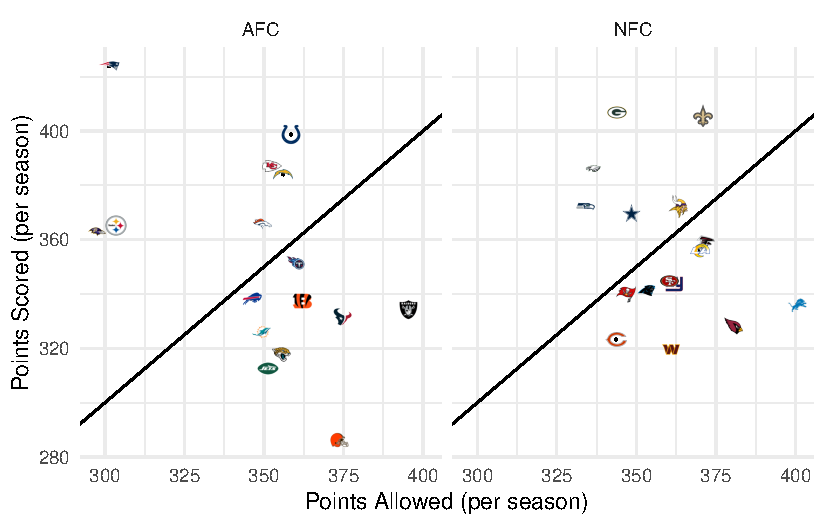
\includegraphics[keepaspectratio]{Final_Project_Team2_files/figure-pdf/fig-effeciency-scatter-plot-1.pdf}}

}

\end{figure}%

\begin{table}

\caption{\label{tbl-effeciency-scatter-plot-AFC}AFC Effeciency tables}

\centering{

\centering
\begin{tabular}{l>{}cccc}
\toprule
Team & image & Average Point Differential & Win Rate & Loss Rate\\
\midrule
NE & \includegraphics[width=0.17in, height=0.17in]{Logos/NE.png} & 122.5833 & 11.2500 & 4.8333\\
PIT & \includegraphics[width=0.17in, height=0.17in]{Logos/PIT.png} & 61.7500 & 10.0417 & 5.9167\\
IND & \includegraphics[width=0.17in, height=0.17in]{Logos/IND.png} & 40.1667 & 9.7500 & 6.2917\\
BAL & \includegraphics[width=0.17in, height=0.17in]{Logos/BAL.png} & 65.3750 & 9.4583 & 6.6250\\
KC & \includegraphics[width=0.17in, height=0.17in]{Logos/KC.png} & 34.5417 & 8.9583 & 7.1250\\
\addlinespace
DEN & \includegraphics[width=0.17in, height=0.17in]{Logos/DEN.png} & 16.2083 & 8.5417 & 7.5417\\
TEN & \includegraphics[width=0.17in, height=0.17in]{Logos/TEN.png} & -8.2917 & 8.4583 & 7.6250\\
LAC & \includegraphics[width=0.17in, height=0.17in]{Logos/LAC.png} & 28.0000 & 8.1667 & 7.9167\\
MIA & \includegraphics[width=0.17in, height=0.17in]{Logos/MIA.png} & -23.2917 & 7.7500 & 8.3333\\
BUF & \includegraphics[width=0.17in, height=0.17in]{Logos/BUF.png} & -8.0000 & 7.7083 & 8.3333\\
\addlinespace
CIN & \includegraphics[width=0.17in, height=0.17in]{Logos/CIN.png} & -24.5833 & 7.2917 & 8.5833\\
NYJ & \includegraphics[width=0.17in, height=0.17in]{Logos/NYJ.png} & -38.5417 & 7.0417 & 9.0417\\
HOU & \includegraphics[width=0.17in, height=0.17in]{Logos/HOU.png} & -43.1905 & 6.7619 & 9.2857\\
LV & \includegraphics[width=0.17in, height=0.17in]{Logos/LV.png} & -61.0417 & 6.5417 & 9.5417\\
JAX & \includegraphics[width=0.17in, height=0.17in]{Logos/JAX.png} & -37.8333 & 6.4167 & 9.6667\\
\addlinespace
CLE & \includegraphics[width=0.17in, height=0.17in]{Logos/CLE.png} & -87.4583 & 5.2917 & 10.7500\\
\bottomrule
\end{tabular}

}

\end{table}%

\begin{table}

\caption{\label{tbl-effeciency-scatter-plot-NFC}NFC Effeciency tables}

\centering{

\centering
\begin{tabular}{l>{}cccc}
\toprule
Team & image & Average Point Differential & Win Rate & Loss Rate\\
\midrule
GB & \includegraphics[width=0.17in, height=0.17in]{Logos/NE.png} & 62.9167 & 9.9583 & 6.0417\\
PHI & \includegraphics[width=0.17in, height=0.17in]{Logos/PIT.png} & 49.7083 & 9.2500 & 6.7500\\
SEA & \includegraphics[width=0.17in, height=0.17in]{Logos/IND.png} & 38.2083 & 9.1250 & 6.9167\\
NO & \includegraphics[width=0.17in, height=0.17in]{Logos/BAL.png} & 34.7083 & 8.9167 & 7.1667\\
DAL & \includegraphics[width=0.17in, height=0.17in]{Logos/KC.png} & 21.4583 & 8.5833 & 7.5000\\
\addlinespace
MIN & \includegraphics[width=0.17in, height=0.17in]{Logos/DEN.png} & 9.2083 & 8.4583 & 7.5417\\
ATL & \includegraphics[width=0.17in, height=0.17in]{Logos/TEN.png} & -13.5417 & 7.7917 & 8.2500\\
LA & \includegraphics[width=0.17in, height=0.17in]{Logos/LAC.png} & -13.8333 & 7.6667 & 8.3750\\
NYG & \includegraphics[width=0.17in, height=0.17in]{Logos/MIA.png} & -18.1250 & 7.6667 & 8.3750\\
CAR & \includegraphics[width=0.17in, height=0.17in]{Logos/BUF.png} & -11.9167 & 7.5833 & 8.4583\\
\addlinespace
SF & \includegraphics[width=0.17in, height=0.17in]{Logos/CIN.png} & -15.7083 & 7.5417 & 8.5000\\
TB & \includegraphics[width=0.17in, height=0.17in]{Logos/NYJ.png} & -6.5417 & 7.5417 & 8.5417\\
CHI & \includegraphics[width=0.17in, height=0.17in]{Logos/HOU.png} & -20.3333 & 7.5000 & 8.5833\\
ARI & \includegraphics[width=0.17in, height=0.17in]{Logos/LV.png} & -52.2083 & 6.9167 & 9.0833\\
WAS & \includegraphics[width=0.17in, height=0.17in]{Logos/JAX.png} & -41.2500 & 6.8333 & 9.1667\\
\addlinespace
DET & \includegraphics[width=0.17in, height=0.17in]{Logos/CLE.png} & -64.5417 & 5.7917 & 10.2083\\
\bottomrule
\end{tabular}

}

\end{table}%

\newpage{}

\#Code Appendix

\begin{Shaded}
\begin{Highlighting}[]
\CommentTok{\#Tidyverse Coding Styling}


\FunctionTok{library}\NormalTok{(tidyverse)}
\FunctionTok{library}\NormalTok{(ggimage)}
\FunctionTok{library}\NormalTok{(kableExtra)}
\FunctionTok{library}\NormalTok{(patchwork)}
\FunctionTok{library}\NormalTok{(ggpubr)}

\NormalTok{NFL\_raw }\OtherTok{\textless{}{-}} \FunctionTok{read.csv}\NormalTok{(}\StringTok{"nfl{-}team{-}statistics (1).csv"}\NormalTok{)}

\NormalTok{NFC\_East\_data }\OtherTok{\textless{}{-}}\NormalTok{ NFL\_raw }\SpecialCharTok{\%\textgreater{}\%}
  \FunctionTok{filter}\NormalTok{(team }\SpecialCharTok{\%in\%} \FunctionTok{c}\NormalTok{(}\StringTok{"DAL"}\NormalTok{, }\StringTok{"NYG"}\NormalTok{, }\StringTok{"PHI"}\NormalTok{, }\StringTok{"WAS"}\NormalTok{))}\SpecialCharTok{\%\textgreater{}\%}
  \FunctionTok{mutate}\NormalTok{(}\AttributeTok{Conf =} \StringTok{\textquotesingle{}NFC\_East\textquotesingle{}}\NormalTok{)}

\NormalTok{NFC\_West\_data }\OtherTok{\textless{}{-}}\NormalTok{ NFL\_raw }\SpecialCharTok{\%\textgreater{}\%}
  \FunctionTok{filter}\NormalTok{(team }\SpecialCharTok{\%in\%} \FunctionTok{c}\NormalTok{(}\StringTok{"LA"}\NormalTok{, }\StringTok{"SEA"}\NormalTok{, }\StringTok{"SF"}\NormalTok{, }\StringTok{"ARI"}\NormalTok{))}\SpecialCharTok{\%\textgreater{}\%}
  \FunctionTok{mutate}\NormalTok{(}\AttributeTok{Conf =} \StringTok{\textquotesingle{}NFC\_West\textquotesingle{}}\NormalTok{)}

\NormalTok{NFC\_North\_data }\OtherTok{\textless{}{-}}\NormalTok{ NFL\_raw }\SpecialCharTok{\%\textgreater{}\%}
  \FunctionTok{filter}\NormalTok{(team }\SpecialCharTok{\%in\%} \FunctionTok{c}\NormalTok{(}\StringTok{"CHI"}\NormalTok{, }\StringTok{"GB"}\NormalTok{, }\StringTok{"DET"}\NormalTok{, }\StringTok{"MIN"}\NormalTok{))}\SpecialCharTok{\%\textgreater{}\%}
  \FunctionTok{mutate}\NormalTok{(}\AttributeTok{Conf =} \StringTok{\textquotesingle{}NFC\_North\textquotesingle{}}\NormalTok{)}

\NormalTok{NFC\_South\_data }\OtherTok{\textless{}{-}}\NormalTok{ NFL\_raw }\SpecialCharTok{\%\textgreater{}\%}
  \FunctionTok{filter}\NormalTok{(team }\SpecialCharTok{\%in\%} \FunctionTok{c}\NormalTok{(}\StringTok{"TB"}\NormalTok{, }\StringTok{"CAR"}\NormalTok{, }\StringTok{"ATL"}\NormalTok{, }\StringTok{"NO"}\NormalTok{))}\SpecialCharTok{\%\textgreater{}\%}
  \FunctionTok{mutate}\NormalTok{(}\AttributeTok{Conf =} \StringTok{\textquotesingle{}NFC\_South\textquotesingle{}}\NormalTok{)}

\NormalTok{AFC\_East\_data }\OtherTok{\textless{}{-}}\NormalTok{ NFL\_raw }\SpecialCharTok{\%\textgreater{}\%}
  \FunctionTok{filter}\NormalTok{(team }\SpecialCharTok{\%in\%} \FunctionTok{c}\NormalTok{(}\StringTok{"NE"}\NormalTok{, }\StringTok{"BUF"}\NormalTok{, }\StringTok{"MIA"}\NormalTok{, }\StringTok{"NYJ"}\NormalTok{))}\SpecialCharTok{\%\textgreater{}\%}
  \FunctionTok{mutate}\NormalTok{(}\AttributeTok{Conf =} \StringTok{\textquotesingle{}AFC\_East\textquotesingle{}}\NormalTok{)}

\NormalTok{AFC\_West\_data }\OtherTok{\textless{}{-}}\NormalTok{ NFL\_raw }\SpecialCharTok{\%\textgreater{}\%}
  \FunctionTok{filter}\NormalTok{(team }\SpecialCharTok{\%in\%} \FunctionTok{c}\NormalTok{(}\StringTok{"DEN"}\NormalTok{, }\StringTok{"LAC"}\NormalTok{, }\StringTok{"KC"}\NormalTok{, }\StringTok{"LV"}\NormalTok{))}\SpecialCharTok{\%\textgreater{}\%}
  \FunctionTok{mutate}\NormalTok{(}\AttributeTok{Conf =} \StringTok{\textquotesingle{}AFC\_West\textquotesingle{}}\NormalTok{)}

\NormalTok{AFC\_North\_data }\OtherTok{\textless{}{-}}\NormalTok{ NFL\_raw }\SpecialCharTok{\%\textgreater{}\%}
  \FunctionTok{filter}\NormalTok{(team }\SpecialCharTok{\%in\%} \FunctionTok{c}\NormalTok{(}\StringTok{"BAL"}\NormalTok{, }\StringTok{"PIT"}\NormalTok{, }\StringTok{"CIN"}\NormalTok{, }\StringTok{"CLE"}\NormalTok{))}\SpecialCharTok{\%\textgreater{}\%}
  \FunctionTok{mutate}\NormalTok{(}\AttributeTok{Conf =} \StringTok{\textquotesingle{}AFC\_North\textquotesingle{}}\NormalTok{)}

\NormalTok{AFC\_South\_data }\OtherTok{\textless{}{-}}\NormalTok{ NFL\_raw }\SpecialCharTok{\%\textgreater{}\%}
  \FunctionTok{filter}\NormalTok{(team }\SpecialCharTok{\%in\%} \FunctionTok{c}\NormalTok{(}\StringTok{"JAX"}\NormalTok{, }\StringTok{"IND"}\NormalTok{, }\StringTok{"HOU"}\NormalTok{, }\StringTok{"TEN"}\NormalTok{))}\SpecialCharTok{\%\textgreater{}\%}
  \FunctionTok{mutate}\NormalTok{(}\AttributeTok{Conf =} \StringTok{\textquotesingle{}AFC\_South\textquotesingle{}}\NormalTok{)}

\NormalTok{NFL\_Clean }\OtherTok{\textless{}{-}} \FunctionTok{bind\_rows}\NormalTok{(NFC\_East\_data, NFC\_North\_data, NFC\_South\_data, NFC\_West\_data, AFC\_East\_data, AFC\_South\_data, AFC\_North\_data, AFC\_West\_data) }\SpecialCharTok{\%\textgreater{}\%}
  \FunctionTok{arrange}\NormalTok{(season, team)}\SpecialCharTok{\%\textgreater{}\%}
    \FunctionTok{separate\_wider\_delim}\NormalTok{(}
    \AttributeTok{cols =} \StringTok{\textquotesingle{}Conf\textquotesingle{}}\NormalTok{,}
    \AttributeTok{delim =} \StringTok{\textquotesingle{}\_\textquotesingle{}}\NormalTok{,}
    \AttributeTok{names =} \FunctionTok{c}\NormalTok{(}\StringTok{\textquotesingle{}Conf\textquotesingle{}}\NormalTok{, }\StringTok{\textquotesingle{}Div\textquotesingle{}}\NormalTok{)}
\NormalTok{  )}

\CommentTok{\#|label: fig{-}Win{-}association}
\CommentTok{\#|fig{-}cap: "Win Association of Offensive and Defensive Pass Yards"}
\CommentTok{\#| fig{-}subcap: }
\CommentTok{\#|   {-} "first"}
\CommentTok{\#|   {-} "second"}
\CommentTok{\#|   {-} "third"}
\CommentTok{\#|   {-} "fourth"}
\CommentTok{\#|fig{-}alt: "Four scatter plots showing NFL data, with axes for wins and various yard metrics. Trend lines suggest correlations."}

\CommentTok{\#author: Timothy Smith}
\NormalTok{plot1}\OtherTok{\textless{}{-}}\NormalTok{NFL\_Clean}\SpecialCharTok{\%\textgreater{}\%}
  \FunctionTok{group\_by}\NormalTok{(Div)}\SpecialCharTok{\%\textgreater{}\%}
\FunctionTok{ggplot}\NormalTok{(}
    \AttributeTok{mapping =} \FunctionTok{aes}\NormalTok{(}
      \AttributeTok{x =}\NormalTok{ offense\_total\_yards\_gained\_pass,}
      \AttributeTok{y =}\NormalTok{ wins,}
      \AttributeTok{color =}\NormalTok{ Conf}
\NormalTok{    )}
\NormalTok{  ) }\SpecialCharTok{+}
  \FunctionTok{geom\_point}\NormalTok{(}\AttributeTok{size =} \DecValTok{1}\NormalTok{, }\AttributeTok{alpha=}\FloatTok{0.2}\NormalTok{) }\SpecialCharTok{+}
  \FunctionTok{labs}\NormalTok{(}\CommentTok{\#Step 4: add labels and title to the data visualization and create the colors for the points{-}{-}{-}{-}}
    \AttributeTok{x =} \StringTok{"Offensive Pass Yards"}\NormalTok{,}
    \AttributeTok{y =} \StringTok{"Wins"}\NormalTok{,}
    \AttributeTok{color =} \StringTok{"Conference"}\NormalTok{,}
    \AttributeTok{title =} \StringTok{"Wins Compared to Offensive Pass Yards"}
\NormalTok{  ) }\SpecialCharTok{+}
  \FunctionTok{scale\_color\_manual}\NormalTok{(}
    \AttributeTok{values =} \FunctionTok{c}\NormalTok{(}\StringTok{"red"}\NormalTok{, }\StringTok{"blue"}\NormalTok{)}
\NormalTok{  )}\SpecialCharTok{+}
  \FunctionTok{theme\_bw}\NormalTok{() }\SpecialCharTok{+}
  \FunctionTok{theme}\NormalTok{(}
    \AttributeTok{legend.position =} \StringTok{"bottom"}
\NormalTok{  )}\SpecialCharTok{+}
  \FunctionTok{geom\_smooth}\NormalTok{(}\AttributeTok{method =} \StringTok{"lm"}\NormalTok{, }\AttributeTok{se =} \ConstantTok{FALSE}\NormalTok{, }\AttributeTok{color =} \StringTok{"black"}\NormalTok{) }

\NormalTok{  plot2}\OtherTok{\textless{}{-}}\NormalTok{NFL\_Clean}\SpecialCharTok{\%\textgreater{}\%}
  \FunctionTok{group\_by}\NormalTok{(Div)}\SpecialCharTok{\%\textgreater{}\%}
\FunctionTok{ggplot}\NormalTok{(}
    \AttributeTok{mapping =} \FunctionTok{aes}\NormalTok{(}
      \AttributeTok{x =}\NormalTok{ offense\_total\_yards\_gained\_run,}
      \AttributeTok{y =}\NormalTok{ wins,}
      \AttributeTok{color =}\NormalTok{ Conf}
\NormalTok{    )}
\NormalTok{  ) }\SpecialCharTok{+}
  \FunctionTok{geom\_point}\NormalTok{(}\AttributeTok{size=}\DecValTok{1}\NormalTok{, }\AttributeTok{alpha=}\FloatTok{0.2}\NormalTok{) }\SpecialCharTok{+}
  \FunctionTok{labs}\NormalTok{(}\CommentTok{\#Step 5: add labels and title to the data visualization and create the colors for the points{-}{-}{-}{-}}
    \AttributeTok{x =} \StringTok{"Offensive Run Yards"}\NormalTok{,}
    \AttributeTok{y =} \StringTok{"Wins"}\NormalTok{,}
    \AttributeTok{color =} \StringTok{"Conference"}\NormalTok{,}
    \AttributeTok{shape =} \StringTok{"team"}\NormalTok{,}
    \AttributeTok{title =} \StringTok{"Wins Compared to Offensive Run Yards"}
\NormalTok{  ) }\SpecialCharTok{+}
  \FunctionTok{scale\_color\_manual}\NormalTok{(}
    \AttributeTok{values =} \FunctionTok{c}\NormalTok{(}\StringTok{"red"}\NormalTok{, }\StringTok{"blue"}\NormalTok{)}
\NormalTok{  )}\SpecialCharTok{+}
  \FunctionTok{theme\_bw}\NormalTok{() }\SpecialCharTok{+}
  \FunctionTok{theme}\NormalTok{(}
    \AttributeTok{legend.position =} \StringTok{"bottom"}
\NormalTok{  )}\SpecialCharTok{+}
  \FunctionTok{geom\_smooth}\NormalTok{(}\AttributeTok{method =} \StringTok{"lm"}\NormalTok{, }\AttributeTok{se =} \ConstantTok{FALSE}\NormalTok{, }\AttributeTok{color =} \StringTok{"black"}\NormalTok{) }
  
\NormalTok{  plot3}\OtherTok{\textless{}{-}}\NormalTok{NFL\_Clean}\SpecialCharTok{\%\textgreater{}\%}
  \FunctionTok{group\_by}\NormalTok{(Div)}\SpecialCharTok{\%\textgreater{}\%}
\FunctionTok{ggplot}\NormalTok{(}
    \AttributeTok{mapping =} \FunctionTok{aes}\NormalTok{(}
      \AttributeTok{x =}\NormalTok{ defense\_total\_yards\_gained\_pass,}
      \AttributeTok{y =}\NormalTok{ wins,}
      \AttributeTok{color =}\NormalTok{ Conf}
\NormalTok{    )}
\NormalTok{  ) }\SpecialCharTok{+}
  \FunctionTok{geom\_point}\NormalTok{(}\AttributeTok{size=}\DecValTok{1}\NormalTok{, }\AttributeTok{alpha=}\FloatTok{0.2}\NormalTok{) }\SpecialCharTok{+}
  \FunctionTok{labs}\NormalTok{(}\CommentTok{\#Step 6: add labels and title to the data visualization and create the colors for the lines{-}{-}{-}{-}}
    \AttributeTok{x =} \StringTok{"Defensive Allowed Pass Yards"}\NormalTok{,}
    \AttributeTok{y =} \StringTok{"Wins"}\NormalTok{,}
    \AttributeTok{color =} \StringTok{"Conference"}\NormalTok{,}
    \AttributeTok{title =} \StringTok{"Wins Compared to Defensive Allowed Pass Yards"}
\NormalTok{  ) }\SpecialCharTok{+}
  \FunctionTok{scale\_color\_manual}\NormalTok{(}
    \AttributeTok{values =} \FunctionTok{c}\NormalTok{(}\StringTok{"red"}\NormalTok{, }\StringTok{"blue"}\NormalTok{)}
\NormalTok{  )}\SpecialCharTok{+}
  \FunctionTok{theme\_bw}\NormalTok{() }\SpecialCharTok{+}
  \FunctionTok{theme}\NormalTok{(}
    \AttributeTok{legend.position =} \StringTok{"bottom"}
\NormalTok{  )}\SpecialCharTok{+}
  \FunctionTok{geom\_smooth}\NormalTok{(}\AttributeTok{method =} \StringTok{"lm"}\NormalTok{, }\AttributeTok{se =} \ConstantTok{FALSE}\NormalTok{, }\AttributeTok{color =} \StringTok{"black"}\NormalTok{) }
  

\NormalTok{  plot4}\OtherTok{\textless{}{-}}\NormalTok{NFL\_Clean}\SpecialCharTok{\%\textgreater{}\%}
  \FunctionTok{group\_by}\NormalTok{(Div)}\SpecialCharTok{\%\textgreater{}\%}
\FunctionTok{ggplot}\NormalTok{(}
    \AttributeTok{mapping =} \FunctionTok{aes}\NormalTok{(}
      \AttributeTok{x =}\NormalTok{ defense\_total\_yards\_gained\_run,}
      \AttributeTok{y =}\NormalTok{ wins,}
      \AttributeTok{color =}\NormalTok{ Conf}
\NormalTok{    )}
\NormalTok{  ) }\SpecialCharTok{+}
  \FunctionTok{geom\_point}\NormalTok{(}\AttributeTok{size=}\DecValTok{1}\NormalTok{, }\AttributeTok{alpha=}\FloatTok{0.2}\NormalTok{) }\SpecialCharTok{+}
  \FunctionTok{labs}\NormalTok{(}\CommentTok{\#Step 7: add labels and title to the data visualization and create the colors for the lines{-}{-}{-}{-}}
    \AttributeTok{x =} \StringTok{"Defensive Allowed Run Yards"}\NormalTok{,}
    \AttributeTok{y =} \StringTok{"Wins"}\NormalTok{,}
    \AttributeTok{color =} \StringTok{"Conference"}\NormalTok{,}
    \AttributeTok{title =} \StringTok{"Wins Compared to Defensive Allowed Run Yards"}
\NormalTok{  ) }\SpecialCharTok{+}
  \FunctionTok{scale\_color\_manual}\NormalTok{(}
    \AttributeTok{values =} \FunctionTok{c}\NormalTok{(}\StringTok{"red"}\NormalTok{, }\StringTok{"blue"}\NormalTok{)}
\NormalTok{  )}\SpecialCharTok{+}
  \FunctionTok{theme\_bw}\NormalTok{() }\SpecialCharTok{+}
  \FunctionTok{theme}\NormalTok{(}
    \AttributeTok{legend.position =} \StringTok{"bottom"}
\NormalTok{  )}\SpecialCharTok{+}
  \FunctionTok{geom\_smooth}\NormalTok{(}\AttributeTok{method =} \StringTok{"lm"}\NormalTok{, }\AttributeTok{se =} \ConstantTok{FALSE}\NormalTok{, }\AttributeTok{color =} \StringTok{"black"}\NormalTok{) }
  
  \FunctionTok{ggarrange}\NormalTok{(plot1, plot2, plot3, plot4, }\AttributeTok{nrow =} \DecValTok{2}\NormalTok{, }\AttributeTok{ncol =} \DecValTok{2}\NormalTok{, }\AttributeTok{common.legend =} \ConstantTok{TRUE}\NormalTok{, }\AttributeTok{legend =} \StringTok{"bottom"}\NormalTok{ )}
  



\CommentTok{\#|tbl{-}cap: "NFL Offensive and Drfensive Statistics"}

\NormalTok{NFL\_O\_D }\OtherTok{\textless{}{-}}\NormalTok{ NFL\_Clean }\SpecialCharTok{\%\textgreater{}\%}
  \FunctionTok{group\_by}\NormalTok{(team)}\SpecialCharTok{\%\textgreater{}\%}
  \FunctionTok{summarize}\NormalTok{(}
    \AttributeTok{Mean\_Wins =} \FunctionTok{mean}\NormalTok{(wins, }\AttributeTok{na.rm =} \ConstantTok{TRUE}\NormalTok{),}
    \AttributeTok{Mean\_O\_pass\_yards =} \FunctionTok{mean}\NormalTok{(offense\_total\_yards\_gained\_pass, }\AttributeTok{na.rm =} \ConstantTok{TRUE}\NormalTok{),}
    \AttributeTok{Mean\_O\_run\_yards =} \FunctionTok{mean}\NormalTok{(offense\_total\_yards\_gained\_run, }\AttributeTok{na.rm =} \ConstantTok{TRUE}\NormalTok{),}
    \AttributeTok{Mean\_D\_pass\_yards =} \FunctionTok{mean}\NormalTok{(defense\_total\_yards\_gained\_pass, }\AttributeTok{na.rm =} \ConstantTok{TRUE}\NormalTok{),}
    \AttributeTok{Mean\_D\_run\_yards =} \FunctionTok{mean}\NormalTok{(defense\_total\_yards\_gained\_run, }\AttributeTok{na.rm =} \ConstantTok{TRUE}\NormalTok{)}
\NormalTok{  ) }
    
    \FunctionTok{names}\NormalTok{(NFL\_O\_D) }\OtherTok{\textless{}{-}} \FunctionTok{c}\NormalTok{(}
    \StringTok{"Teams"}\NormalTok{,}
    \StringTok{"Average Wins"}\NormalTok{,}
    \StringTok{"Mean Offensive Pass Yards"}\NormalTok{,}
    \StringTok{"Mean Offense Run Yards"}\NormalTok{,}
    \StringTok{"Mean Defensive Pass Yards"}\NormalTok{,}
    \StringTok{"Mean Defensive Run Yards"}
\NormalTok{    )}
  
\NormalTok{NFL\_O\_D }\SpecialCharTok{\%\textgreater{}\%}
  \FunctionTok{kable}\NormalTok{(}
    \AttributeTok{booktabs =} \ConstantTok{TRUE}\NormalTok{,}
    \AttributeTok{align =} \FunctionTok{c}\NormalTok{(}\StringTok{"l"}\NormalTok{, }\FunctionTok{rep}\NormalTok{(}\StringTok{"c"}\NormalTok{,}\DecValTok{10}\NormalTok{)))}

\CommentTok{\#author: Isaac Swope}


\FunctionTok{ggplot}\NormalTok{(NFL\_Clean) }\SpecialCharTok{+}
  \FunctionTok{aes}\NormalTok{(}\AttributeTok{x =} \FunctionTok{fct\_reorder}\NormalTok{(team, wins, }\AttributeTok{.fun=}\NormalTok{sum, }\AttributeTok{.desc=}\ConstantTok{TRUE}\NormalTok{), }\AttributeTok{y =}\NormalTok{ wins, }\AttributeTok{fill =}\NormalTok{ Conf) }\SpecialCharTok{+}
  \FunctionTok{geom\_col}\NormalTok{(}\AttributeTok{color =} \ConstantTok{NA}\NormalTok{) }\SpecialCharTok{+}
  \FunctionTok{facet\_wrap}\NormalTok{(}\StringTok{"Div"}\NormalTok{, }\AttributeTok{scales =} \StringTok{"free"}\NormalTok{) }\SpecialCharTok{+} \CommentTok{\#eliminate spacing between columns due to scale}
  \FunctionTok{labs}\NormalTok{(}\AttributeTok{y =} \StringTok{"Wins"}\NormalTok{, }
       \AttributeTok{x =} \StringTok{"Teams"}\NormalTok{,}
\NormalTok{       )}
  
\CommentTok{\#author: Isaac Swope}

\NormalTok{winsTable }\OtherTok{\textless{}{-}}\NormalTok{ NFL\_Clean }\SpecialCharTok{\%\textgreater{}\%}
  \FunctionTok{group\_by}\NormalTok{(team)}\SpecialCharTok{\%\textgreater{}\%}
  \FunctionTok{summarize}\NormalTok{(}
    \AttributeTok{Count=}\FunctionTok{n}\NormalTok{(),}
    \AttributeTok{Min =} \FunctionTok{min}\NormalTok{(wins, }\AttributeTok{na.rm =} \ConstantTok{TRUE}\NormalTok{),}
    \AttributeTok{Quartile\_1 =} \FunctionTok{quantile}\NormalTok{(wins, }\AttributeTok{probs =} \FloatTok{0.25}\NormalTok{, }\AttributeTok{na.rm =} \ConstantTok{TRUE}\NormalTok{),}
    \AttributeTok{Median =} \FunctionTok{median}\NormalTok{(wins, }\AttributeTok{na.rm =} \ConstantTok{TRUE}\NormalTok{),}
    \AttributeTok{Quintile\_3 =} \FunctionTok{quantile}\NormalTok{(wins, }\AttributeTok{probs =} \FloatTok{0.75}\NormalTok{, }\AttributeTok{na.rm =} \ConstantTok{TRUE}\NormalTok{),}
    \AttributeTok{Max =} \FunctionTok{max}\NormalTok{(wins, }\AttributeTok{na.rm =} \ConstantTok{TRUE}\NormalTok{),}
    \AttributeTok{Mean =} \FunctionTok{mean}\NormalTok{(wins, }\AttributeTok{na.rm =} \ConstantTok{TRUE}\NormalTok{),}
    \AttributeTok{SD =} \FunctionTok{sd}\NormalTok{(wins, }\AttributeTok{na.rm =} \ConstantTok{TRUE}\NormalTok{),}
\NormalTok{  )}\SpecialCharTok{\%\textgreater{}\%}
  \FunctionTok{mutate}\NormalTok{(}
    \FunctionTok{across}\NormalTok{(}
      \AttributeTok{.cols =} \FunctionTok{where}\NormalTok{(is.numeric),}
      \AttributeTok{.fns =} \SpecialCharTok{\textasciitilde{}}\FunctionTok{round}\NormalTok{(.x, }\AttributeTok{digits =} \DecValTok{2}\NormalTok{)}
\NormalTok{    )}
\NormalTok{  )}

\FunctionTok{names}\NormalTok{(winsTable) }\OtherTok{\textless{}{-}} \FunctionTok{c}\NormalTok{(}
    \StringTok{"Team"}\NormalTok{,}
    \StringTok{"Seasons"}\NormalTok{,}
    \StringTok{"Minimum"}\NormalTok{,}
    \StringTok{"Quartile 1"}\NormalTok{,}
    \StringTok{"Median"}\NormalTok{,}
    \StringTok{"Quartile 3"}\NormalTok{,}
    \StringTok{"Max"}\NormalTok{,}
    \StringTok{"Mean"}\NormalTok{,}
    \StringTok{"SD"}
\NormalTok{    )}
  
\NormalTok{winsTable }\SpecialCharTok{\%\textgreater{}\%}
  \FunctionTok{kable}\NormalTok{(}
    \AttributeTok{booktabs =} \ConstantTok{TRUE}\NormalTok{,}
    \AttributeTok{align =} \FunctionTok{c}\NormalTok{(}\StringTok{"l"}\NormalTok{, }\FunctionTok{rep}\NormalTok{(}\StringTok{"c"}\NormalTok{,}\DecValTok{10}\NormalTok{))}
\NormalTok{  )}

\NormalTok{NFL\_Clean\_3 }\OtherTok{\textless{}{-}}\NormalTok{ NFL\_Clean }\SpecialCharTok{\%\textgreater{}\%}
  \FunctionTok{select}\NormalTok{(team, Conf, score\_differential, points\_scored,}
\NormalTok{         points\_allowed, wins, losses) }\SpecialCharTok{\%\textgreater{}\%}
  \FunctionTok{group\_by}\NormalTok{(team, Conf) }\SpecialCharTok{\%\textgreater{}\%}
  \FunctionTok{summarise}\NormalTok{(}
    \AttributeTok{points\_scored =} \FunctionTok{mean}\NormalTok{(points\_scored),}
    \AttributeTok{points\_allowed =} \FunctionTok{mean}\NormalTok{(points\_allowed),}
    \AttributeTok{wins =} \FunctionTok{mean}\NormalTok{(wins),}
    \AttributeTok{losses =} \FunctionTok{mean}\NormalTok{(losses),}
    \AttributeTok{point\_differential =} \FunctionTok{mean}\NormalTok{(score\_differential),}
    \AttributeTok{.groups =} \StringTok{"drop"}
\NormalTok{  )}
\NormalTok{NFL\_Clean\_3}\SpecialCharTok{$}\NormalTok{logo }\OtherTok{\textless{}{-}} \FunctionTok{paste0}\NormalTok{(}\StringTok{"Logos/"}\NormalTok{, NFL\_Clean\_3}\SpecialCharTok{$}\NormalTok{team, }\StringTok{".png"}\NormalTok{)}

\FunctionTok{ggplot}\NormalTok{(NFL\_Clean\_3) }\SpecialCharTok{+}
  \FunctionTok{aes}\NormalTok{(}\AttributeTok{x =}\NormalTok{ points\_allowed, }\AttributeTok{y =}\NormalTok{ points\_scored) }\SpecialCharTok{+}
  \FunctionTok{geom\_point}\NormalTok{(}\AttributeTok{size =} \FloatTok{0.1}\NormalTok{) }\SpecialCharTok{+}
  \FunctionTok{geom\_image}\NormalTok{(}\FunctionTok{aes}\NormalTok{(}\AttributeTok{image =}\NormalTok{ logo)) }\SpecialCharTok{+}
  \FunctionTok{labs}\NormalTok{(}
    \AttributeTok{x =} \StringTok{"Points Allowed (per season)"}\NormalTok{,}
    \AttributeTok{y =} \StringTok{"Points Scored (per season)"}
\NormalTok{  ) }\SpecialCharTok{+}
  \FunctionTok{geom\_abline}\NormalTok{(}\AttributeTok{slope =} \DecValTok{1}\NormalTok{, }\AttributeTok{intercept =} \DecValTok{0}\NormalTok{) }\SpecialCharTok{+}
  \FunctionTok{theme\_minimal}\NormalTok{() }\SpecialCharTok{+}
  \FunctionTok{facet\_wrap}\NormalTok{(}\FunctionTok{vars}\NormalTok{(Conf))}

\NormalTok{AFC\_table }\OtherTok{\textless{}{-}}\NormalTok{ NFL\_Clean\_3}\SpecialCharTok{\%\textgreater{}\%}
  \FunctionTok{filter}\NormalTok{(Conf }\SpecialCharTok{==} \StringTok{\textquotesingle{}AFC\textquotesingle{}}\NormalTok{)}\SpecialCharTok{\%\textgreater{}\%}
  \FunctionTok{select}\NormalTok{(team, point\_differential, wins, losses, logo)}\SpecialCharTok{\%\textgreater{}\%}
  \FunctionTok{mutate}\NormalTok{(}
    \AttributeTok{point\_differential =} \FunctionTok{round}\NormalTok{(point\_differential, }\AttributeTok{digits =} \DecValTok{4}\NormalTok{),}
    \AttributeTok{wins =} \FunctionTok{round}\NormalTok{(wins, }\AttributeTok{digits =} \DecValTok{4}\NormalTok{),}
    \AttributeTok{losses =} \FunctionTok{round}\NormalTok{(losses, }\AttributeTok{digits =} \DecValTok{4}\NormalTok{),}
    \AttributeTok{image =} \StringTok{""}
\NormalTok{  )}\SpecialCharTok{\%\textgreater{}\%}
  \FunctionTok{arrange}\NormalTok{(}\FunctionTok{desc}\NormalTok{(wins)) }\SpecialCharTok{\%\textgreater{}\%}
  \FunctionTok{rename}\NormalTok{(}
    \AttributeTok{Team =}\NormalTok{ team,}
    \StringTok{\textasciigrave{}}\AttributeTok{Average Point Differential}\StringTok{\textasciigrave{}} \OtherTok{=}\NormalTok{ point\_differential,}
    \StringTok{\textasciigrave{}}\AttributeTok{Win Rate}\StringTok{\textasciigrave{}} \OtherTok{=}\NormalTok{ wins,}
    \StringTok{\textasciigrave{}}\AttributeTok{Loss Rate}\StringTok{\textasciigrave{}} \OtherTok{=}\NormalTok{ losses}
\NormalTok{  )}

\NormalTok{AFC\_table }\SpecialCharTok{\%\textgreater{}\%}
  \FunctionTok{select}\NormalTok{(Team, image, }\StringTok{\textasciigrave{}}\AttributeTok{Average Point Differential}\StringTok{\textasciigrave{}}\NormalTok{, }\StringTok{\textasciigrave{}}\AttributeTok{Win Rate}\StringTok{\textasciigrave{}}\NormalTok{, }\StringTok{\textasciigrave{}}\AttributeTok{Loss Rate}\StringTok{\textasciigrave{}}\NormalTok{) }\SpecialCharTok{\%\textgreater{}\%}
  \FunctionTok{kable}\NormalTok{(}
    \AttributeTok{booktabs =} \ConstantTok{TRUE}\NormalTok{,}
    \AttributeTok{align =} \FunctionTok{c}\NormalTok{(}\StringTok{"l"}\NormalTok{, }\FunctionTok{rep}\NormalTok{(}\StringTok{"c"}\NormalTok{, }\DecValTok{10}\NormalTok{)),}
    \AttributeTok{format =} \StringTok{"latex"}
\NormalTok{  )}\SpecialCharTok{\%\textgreater{}\%}
  \FunctionTok{kable\_paper}\NormalTok{()}\SpecialCharTok{\%\textgreater{}\%}
  \FunctionTok{column\_spec}\NormalTok{(}\DecValTok{2}\NormalTok{, }\AttributeTok{image =} \FunctionTok{spec\_image}\NormalTok{(}\AttributeTok{path =}\NormalTok{ AFC\_table}\SpecialCharTok{$}\NormalTok{logo, }\DecValTok{50}\NormalTok{, }\DecValTok{50}\NormalTok{))}

\NormalTok{NFC\_table }\OtherTok{\textless{}{-}}\NormalTok{ NFL\_Clean\_3}\SpecialCharTok{\%\textgreater{}\%}
  \FunctionTok{filter}\NormalTok{(Conf }\SpecialCharTok{==} \StringTok{\textquotesingle{}NFC\textquotesingle{}}\NormalTok{)}\SpecialCharTok{\%\textgreater{}\%}
  \FunctionTok{select}\NormalTok{(team, point\_differential, wins, losses, logo)}\SpecialCharTok{\%\textgreater{}\%}
  \FunctionTok{mutate}\NormalTok{(}
    \AttributeTok{point\_differential =} \FunctionTok{round}\NormalTok{(point\_differential, }\AttributeTok{digits =} \DecValTok{4}\NormalTok{),}
    \AttributeTok{wins =} \FunctionTok{round}\NormalTok{(wins, }\AttributeTok{digits =} \DecValTok{4}\NormalTok{),}
    \AttributeTok{losses =} \FunctionTok{round}\NormalTok{(losses, }\AttributeTok{digits =} \DecValTok{4}\NormalTok{),}
    \AttributeTok{image =} \StringTok{""}
\NormalTok{  )}\SpecialCharTok{\%\textgreater{}\%}
  \FunctionTok{arrange}\NormalTok{(}\FunctionTok{desc}\NormalTok{(wins)) }\SpecialCharTok{\%\textgreater{}\%}
  \FunctionTok{rename}\NormalTok{(}
    \AttributeTok{Team =}\NormalTok{ team,}
    \StringTok{\textasciigrave{}}\AttributeTok{Average Point Differential}\StringTok{\textasciigrave{}} \OtherTok{=}\NormalTok{ point\_differential,}
    \StringTok{\textasciigrave{}}\AttributeTok{Win Rate}\StringTok{\textasciigrave{}} \OtherTok{=}\NormalTok{ wins,}
    \StringTok{\textasciigrave{}}\AttributeTok{Loss Rate}\StringTok{\textasciigrave{}} \OtherTok{=}\NormalTok{ losses}
\NormalTok{  )}

\NormalTok{NFC\_table }\SpecialCharTok{\%\textgreater{}\%}
  \FunctionTok{select}\NormalTok{(Team, image, }\StringTok{\textasciigrave{}}\AttributeTok{Average Point Differential}\StringTok{\textasciigrave{}}\NormalTok{, }\StringTok{\textasciigrave{}}\AttributeTok{Win Rate}\StringTok{\textasciigrave{}}\NormalTok{, }\StringTok{\textasciigrave{}}\AttributeTok{Loss Rate}\StringTok{\textasciigrave{}}\NormalTok{) }\SpecialCharTok{\%\textgreater{}\%}
  \FunctionTok{kable}\NormalTok{(}
    \AttributeTok{booktabs =} \ConstantTok{TRUE}\NormalTok{,}
    \AttributeTok{align =} \FunctionTok{c}\NormalTok{(}\StringTok{"l"}\NormalTok{, }\FunctionTok{rep}\NormalTok{(}\StringTok{"c"}\NormalTok{, }\DecValTok{10}\NormalTok{)),}
    \AttributeTok{format =} \StringTok{"latex"}
\NormalTok{  )}\SpecialCharTok{\%\textgreater{}\%}
  \FunctionTok{kable\_paper}\NormalTok{()}\SpecialCharTok{\%\textgreater{}\%}
  \FunctionTok{column\_spec}\NormalTok{(}\DecValTok{2}\NormalTok{, }\AttributeTok{image =} \FunctionTok{spec\_image}\NormalTok{(}\AttributeTok{path =}\NormalTok{ AFC\_table}\SpecialCharTok{$}\NormalTok{logo, }\DecValTok{50}\NormalTok{, }\DecValTok{50}\NormalTok{))}
\end{Highlighting}
\end{Shaded}





\end{document}
